\documentclass[journal]{IEEEtran}
\usepackage{amsmath,amssymb,mathtools,bm}
\usepackage{booktabs,array,multirow}
\usepackage{graphicx}
\usepackage[caption=false,font=footnotesize]{subfig}
\usepackage{cite}
\usepackage{url}
\usepackage{microtype}
\usepackage{balance}
\usepackage{tikz}
\usetikzlibrary{arrows.meta,positioning,fit}
\usepackage[hidelinks]{hyperref}
\graphicspath{{figures/}}
\interdisplaylinepenalty=2500
\newcommand{\R}{\mathrm{R}}
\newcommand{\M}{\mathrm{M}}
\newcommand{\F}{\mathrm{F}}
\newcommand{\given}{\,\middle|\,}
\newcommand{\trans}{\mathsf T}
\newcommand{\vect}[1]{\bm{#1}}
\newcommand{\Prb}{\mathbb P}
\newcommand{\E}{\mathbb E}

\title{A Hidden Markov Framework for Time-to-Flare Prediction in Crohn's Disease Under Endogenous Laboratory Sampling: A Simulation Study}

\author{Rishi Jasti%
\thanks{R. Jasti is with the North Carolina School of Science and Mathematics, Durham, NC, USA (e-mail: jasti27r@ncssm.edu).}}

\begin{document}
\maketitle

\begin{abstract}
We present a hidden Markov framework for longitudinal Crohn's disease monitoring with state-dependent laboratory sampling. The model combines daily Gaussian wearable summaries, intermittent log-normal laboratory biomarkers, and the laboratory-draw indicator in one observation likelihood; laboratory values contribute only on days when a panel is drawn. At each landmark day, we distinguish two mathematically different first-passage quantities: an unconditional distribution that assigns the current flare posterior to day zero, and a transient-conditional distribution whose mean is necessarily bounded by the Remission- and Mild-state hitting-time means. Model parameters are estimated without simulator state labels by Baum--Welch expectation maximization using @@N_STARTS@@ prespecified initializations. A @@N_PARAM_MEMBERS@@-member responsibility-conditioned empirical-Bayes mixture propagates transition, emission, initial-state, and sampling-rate variation through HMM filtering and first-passage calculations; the event-history comparator is evaluated as a separate @@N_HAZARD_MEMBERS@@-member patient-bootstrap ensemble. Evaluation retains administratively censored landmarks, preserves the probability tail beyond the @@N_DAYS@@-day observation window, and uses a censored logarithmic score, fixed-horizon Brier scores, calibration, interval coverage, and sharpness with seed- and patient-clustered uncertainty. Complete landmark PMFs and all fitted model objects are archived. Across ten independent simulations of 120 patients each, the endogenous-sampling HMM obtained a censored log score of @@PROP_NLL@@ (95\% CI @@PROP_NLL_CI@@), a four-horizon mean Brier score of @@PROP_IBS@@ (@@PROP_IBS_CI@@), and @@PROP_COV@@ empirical coverage for nominal 90\% intervals. Its difference from the otherwise identical HMM that ignored the draw indicator was small: @@DIFF_NOLAM_NLL@@ in log score (@@DIFF_NOLAM_NLL_CI@@) and @@DIFF_NOLAM_IBS@@ in mean Brier score (@@DIFF_NOLAM_IBS_CI@@), where positive values favor the endogenous model. The analysis therefore supports the validity of the time-to-flare interface but does not establish a practically important gain from the draw indicator in this well-specified regime. A prespecified sensitivity analysis excluding landmarks already in the flare state is reported separately.
\end{abstract}

\begin{IEEEkeywords}
Crohn's disease, hidden Markov models, informative observation times, missing not at random, first-passage time, survival prediction, calibration, proper scoring rules.
\end{IEEEkeywords}

\section{Introduction}
\IEEEPARstart{C}{rohn's} disease is characterized by transitions among clinically quiescent, mildly active, and flare states. Wearable devices can provide dense physiological measurements, whereas laboratory biomarkers are comparatively accurate but intermittent. The timing of a laboratory panel can itself be informative: patients with greater disease activity may be sampled more often. A monitoring model should therefore use the draw indicator as an observation rather than treating every absent laboratory value as missing at random.

A clinician-facing output should also be more explicit than a per-day flare score. At study day $d$, the relevant quantity is a distribution over the waiting time until the next flare. A subtle but essential distinction arises when the current filter assigns positive probability to the flare state. The unconditional waiting-time law contains an atom at zero; the law conditional on not currently being in flare does not. Their means are different, and only the latter is constrained to lie between the state-specific transient hitting-time means. Failing to distinguish them creates an apparent contradiction whenever a plotted expected waiting time approaches zero while the displayed equation conditions on transient states.

This study makes five contributions.
\begin{enumerate}
\item It specifies one coherent likelihood in which fresh daily wearable observations are Gaussian, laboratory biomarkers are log-normal when observed, and absent laboratory values never enter the emission density.
\item It derives both the unconditional and transient-conditional first-passage distributions, including the day-zero mass and the finite-horizon survival tail.
\item It fits the latent states by expectation maximization rather than using the simulator's true states, and it propagates parameter variation by a transparent responsibility-weighted parameter mixture.
\item It compares the endogenous-sampling HMM with a no-draw-indicator HMM, a narrowly defined draw-stratified-emission HMM, and a discrete-time event-history model on the same time-to-flare output using censoring-aware proper scores and clustered uncertainty.
\item It supplies a one-command reproducibility pipeline, complete PMF archives, serialized HMM and event-history ensembles, generated tables and figures, and acceptance tests linking every reported number to code.
\end{enumerate}

The scope is deliberately limited to a controlled simulation study. No claim of clinical validation is made, and an IBDMDB illustration is not used as confirmatory evidence because its scheduled blood-draw cadence, repeated visits, absence of wearable measurements, and visit-scale timing require a separate clustered and cadence-specific analysis.

\section{Related Work}
\subsection{Informative observation and dropout}
The distinction among missing completely at random, missing at random, and missing not at random is foundational in longitudinal analysis \cite{little_rubin,daniels_hogan}. Diggle and Kenward gave an early selection-model treatment of informative dropout in longitudinal data \cite{diggle}. Informative dropout models commonly connect a longitudinal process and an event process through shared latent structure. Bartolucci and Farcomeni developed a discrete-time event-history extension of latent Markov models with informative dropout \cite{bartolucci2015}, and later a shared-parameter continuous-time hidden Markov and survival model \cite{bartolucci2019}. Marino and Alf\`o used finite mixtures of hidden Markov models to accommodate longitudinal responses subject to dropout \cite{marino2020}. Pandolfi, Bartolucci, and Pennoni considered a continuous-response HMM that accommodates intermittent missingness as well as dropout \cite{pandolfi2023}. These works are directly relevant because they demonstrate how observation or dropout processes can share latent disease structure and how EM recursions can estimate the resulting models.

The present problem differs in one important respect: laboratory non-observation is intermittent rather than terminal. A patient can have no laboratory panel today and a panel later. The Bernoulli draw process is therefore modeled at every day and enters the HMM emission likelihood alongside wearables and observed laboratory values. The conceptual relationship to shared-parameter and event-history models remains close, but the event of interest is disease flare rather than study dropout.

\subsection{Hidden-state disease progression and first-passage prediction}
Forward--backward filtering and Baum--Welch estimation are classical HMM methods \cite{rabiner,cappe}. Absorbing Markov-chain identities provide exact first-passage distributions and means through the transient matrix $Q$ and fundamental matrix $(I-Q)^{-1}$ \cite{kemeny}. Joint longitudinal--event modeling connects evolving biomarkers to event times through shared structure \cite{tsiatis}, while threshold-regression work treats event times as first passage of a stochastic process to a boundary \cite{lee_whitmore}. Related disease-progression work has used hidden-state and semi-Markov models to represent clinical deterioration and absorption risk \cite{alaa,liu_cthmm}. The present framework composes the current filtered state posterior with those classical first-passage identities.

\subsection{Evaluation of probabilistic event-time forecasts}
A predictive distribution should be evaluated by proper scoring rules, calibration, and sharpness rather than by discrimination alone. The Brier score has a standard survival-data extension \cite{graf1999}, and Gneiting and Raftery provide the general theory of proper scores and the calibration--sharpness principle \cite{gneiting2007}. AUROC remains useful for the secondary question of current-state classification, but it does not evaluate the claimed time-to-flare distribution. Longitudinal wearable studies have also reported autonomic changes associated with inflammatory-bowel-disease activity and physiological changes preceding flares \cite{hirten2021,hirten2025}; those findings motivate the monitoring setting but do not constitute validation of the present simulation model.

\section{Model}
\subsection{Latent dynamics and observations}
Let $S_d\in\mathcal S=\{\R,\M,\F\}$ denote the latent disease state on day $d$. The physiological process is a time-homogeneous Markov chain with initial distribution $\vect{\pi}_0$ and transition matrix $P=(P_{ij})$. The flare state is not physiologically absorbing; it is made absorbing only within the landmark-specific first-passage calculation of Section~\ref{sec:hitting}.

Each day produces a wearable vector $Y_d^{(w)}\in\mathbb R^p$, a laboratory-draw indicator $L_d\in\{0,1\}$, and, when $L_d=1$, a positive laboratory vector $Y_d^{(\ell)}\in\mathbb R_+^q$. The observed tuple is
\begin{equation}
O_d=\left(Y_d^{(w)},L_d,L_dY_d^{(\ell)}\right).
\end{equation}
The filtration $\mathcal F_d=\sigma(O_1,\ldots,O_d)$ contains only information available through day $d$.

\subsection{Coherent observation likelihood}
Conditional on $S_d=i$, the wearable channels are independent Gaussian summaries,
\begin{equation}
Y_d^{(w)}\mid S_d=i\sim\mathcal N(\vect{\mu}_i^{(w)},\operatorname{diag}[(\vect{\sigma}_i^{(w)})^2]),
\end{equation}
the draw indicator is Bernoulli,
\begin{equation}
L_d\mid S_d=i\sim\operatorname{Bernoulli}(\lambda_i),
\end{equation}
and each positive laboratory channel is log-normal when observed,
\begin{equation}
\log Y_d^{(\ell)}\mid(S_d=i,L_d=1)
\sim\mathcal N(\vect{\nu}_i,\operatorname{diag}(\vect{\tau}_i^2)).
\end{equation}
The complete day-$d$ emission factor is
\begin{align}
 b_i(O_d)&=\phi_p\!\left(Y_d^{(w)};\vect{\mu}_i^{(w)},\vect{\sigma}_i^{(w)}\right)
 \lambda_i^{L_d}(1-\lambda_i)^{1-L_d} \notag\\
 &\quad\times\left[f_{\mathrm{LN}}\!\left(Y_d^{(\ell)};\vect{\nu}_i,\vect{\tau}_i\right)\right]^{L_d}.
 \label{eq:emission}
\end{align}
Thus, when $L_d=0$, the laboratory-density factor equals one. No forward-filled laboratory value is evaluated in the HMM likelihood. Last-observation-carried-forward values are used only as causal covariates in the separate event-history comparator.

\subsection{Filtering under endogenous sampling}
Let $\pi_d(i)=\Prb(S_d=i\mid\mathcal F_d)$. The prediction and update are
\begin{align}
\pi_{d\mid d-1}(i)&=\sum_{j\in\mathcal S}\pi_{d-1}(j)P_{ji},\\
\pi_d(i)&=\frac{b_i(O_d)\pi_{d\mid d-1}(i)}{\sum_{k\in\mathcal S}b_k(O_d)\pi_{d\mid d-1}(k)}.
\end{align}
On a lab-absent day, posterior odds between states $i$ and $j$ contain the factor
\begin{equation}
\frac{1-\lambda_i}{1-\lambda_j}.
\end{equation}
If $\lambda_i>\lambda_j$, laboratory absence shifts posterior odds away from state $i$. When all $\lambda_i$ are equal, the factor cancels and the model reduces to the no-draw-indicator HMM.

\begin{figure}[t]
\centering
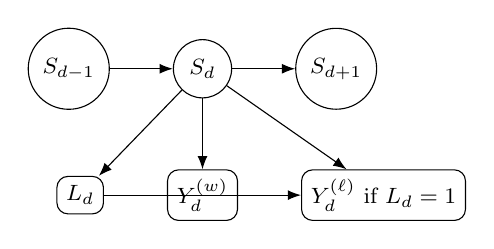
\begin{tikzpicture}[>=Latex, node distance=9mm and 8mm, every node/.style={font=\footnotesize}]
\node[draw,circle,minimum size=7mm] (s1) {$S_{d-1}$};
\node[draw,circle,minimum size=7mm,right=of s1] (s2) {$S_d$};
\node[draw,circle,minimum size=7mm,right=of s2] (s3) {$S_{d+1}$};
\draw[->] (s1)--(s2); \draw[->] (s2)--(s3);
\node[draw,rectangle,rounded corners,below=of s2] (w) {$Y_d^{(w)}$};
\node[draw,rectangle,rounded corners,left=of w] (l) {$L_d$};
\node[draw,rectangle,rounded corners,right=of w] (b) {$Y_d^{(\ell)}$ if $L_d=1$};
\draw[->] (s2)--(w); \draw[->] (s2)--(l); \draw[->] (s2)--(b);
\draw[->] (l)--(b);
\end{tikzpicture}
\caption{Graphical structure at one landmark day. The draw indicator is observed and state-dependent; the laboratory-density term is included only when $L_d=1$.}
\label{fig:graph}
\end{figure}

\section{First-Passage Prediction}\label{sec:hitting}
At every landmark day $d$, define the rolling waiting time
\begin{equation}
H_d=\inf\{n\ge 0:S_{d+n}=\F\}.
\end{equation}
For the first-passage calculation, reorder the states as $(\R,\M,\F)$ and replace the flare row by an absorbing row. Write
\begin{equation}
P^*=\begin{pmatrix}Q&\vect{r}\\\vect{0}^{\trans}&1\end{pmatrix},
\qquad N=(I-Q)^{-1},
\end{equation}
where $Q$ is the $2\times2$ transient block and $\vect{r}$ is the transient-to-flare column. Let
\begin{equation}
\vect{q}_d=(\pi_d(\R),\pi_d(\M))^{\trans}.
\end{equation}

\subsection{Unconditional law}
The complete landmark-specific distribution is
\begin{align}
\Prb(H_d=0\mid\mathcal F_d)&=\pi_d(\F),\label{eq:p0}\\
\Prb(H_d=n\mid\mathcal F_d)&=\vect{q}_d^{\trans}Q^{n-1}\vect{r},
\quad n\ge1,\label{eq:pn}\\
\Prb(H_d>h\mid\mathcal F_d)&=\vect{q}_d^{\trans}Q^h\vect{1}.\label{eq:tail}
\end{align}
The final expression is retained as a tail category in every finite numerical PMF. In particular, the 120-day observation horizon is never used to renormalize the predictive distribution.

The unconditional mean is
\begin{equation}
\E(H_d\mid\mathcal F_d)=\vect{q}_d^{\trans}N\vect{1}.
\label{eq:uncondmean}
\end{equation}
This mean can approach zero because it is multiplied implicitly by the posterior probability of still being in a transient state.

\subsection{Conditional law given no current flare}
When $\vect{q}_d^{\trans}\vect{1}>0$, the transient-conditional mean is
\begin{equation}
\E(H_d\mid\mathcal F_d,S_d\in\{\R,\M\})
=\frac{\vect{q}_d^{\trans}N\vect{1}}{\vect{q}_d^{\trans}\vect{1}}.
\label{eq:condmean}
\end{equation}
Let $m_{\R}=(N\vect{1})_{\R}$ and $m_{\M}=(N\vect{1})_{\M}$. Equation~\eqref{eq:condmean} is a convex combination of $m_{\R}$ and $m_{\M}$, so
\begin{align}
\min(m_{\R},m_{\M})
&\le \E(H_d\mid\mathcal F_d,S_d\in\{\R,\M\}) \notag\\
&\le\max(m_{\R},m_{\M}).
\label{eq:bound}
\end{align}
If the filter assigns zero transient mass, the conditional mean is undefined and is displayed as a gap rather than as zero. This is the exact reconciliation required between a near-zero clinical waiting-time curve and the transient-state bound.

\subsection{Parameter-mixture predictive law}
For parameter draws $\theta^{(0)},\ldots,\theta^{(B)}$, the reported PMF is
\begin{equation}
\widehat p_d(n)=\frac{1}{B+1}\sum_{b=0}^{B}
 p_{\theta^{(b)}}(H_d=n\mid\mathcal F_d),
\end{equation}
with the filtering recursion and first-passage transformation recomputed for every draw. This can widen the predictive distribution when transition, emission, or sampling parameters are uncertain.

\section{Latent-State Estimation and Comparators}
\subsection{Baum--Welch estimation}
The main HMM is fit without access to simulator state labels. For training patient $p$, the forward--backward recursions produce
\begin{align}
\gamma_{pd}(i)&=\Prb(S_{pd}=i\mid O_{p,1:D}),\\
\xi_{pd}(i,j)&=\Prb(S_{pd}=i,S_{p,d+1}=j\mid O_{p,1:D}).
\end{align}
The principal M-step updates are
\begin{align}
\widehat P_{ij}&=
\frac{\sum_{p,d}\xi_{pd}(i,j)+a_{ij}}
{\sum_{p,d}\sum_k\xi_{pd}(i,k)+\sum_k a_{ik}},\label{eq:Pupdate}\\
\widehat\lambda_i&=
\frac{\sum_{p,d}\gamma_{pd}(i)L_{pd}+a_i}
{\sum_{p,d}\gamma_{pd}(i)+a_i+b_i},\label{eq:lamupdate}\\
\widehat{\vect{\nu}}_i&=
\frac{\sum_{p,d}\gamma_{pd}(i)L_{pd}\log Y_{pd}^{(\ell)}}
{\sum_{p,d}\gamma_{pd}(i)L_{pd}},\label{eq:labupdate}
\end{align}
with analogous responsibility-weighted updates for Gaussian wearable means and variances and log-laboratory variances. Weak pseudocounts prevent zero transition and draw probabilities. Initialization uses $K$-means on standardized training wearables; labels are ordered after each fit by increasing wearable-severity score, not by true states. The observed-data log likelihood determines convergence.

\subsection{Parameter uncertainty}
At the final EM solution, responsibility-weighted expected counts are used to construct a reproducible empirical-Bayes approximation. Initial and transition probabilities are drawn from Dirichlet distributions based on expected counts; draw rates are drawn from beta distributions based on expected draw and non-draw counts; independent Gaussian/log-Gaussian means and scales are drawn from weakly regularized normal--scaled-chi-square approximations. @@N_PARAM_DRAWS@@ draws plus the EM estimate are used for each HMM, for @@N_PARAM_MEMBERS@@ mixture members per model. Each primary HMM fit uses @@N_STARTS@@ observable-data initializations and retains every likelihood trace and selection diagnostic. This procedure propagates parameter variation but conditions on the final EM responsibilities; it is therefore not claimed to be an exact fully Bayesian posterior.

\subsection{Comparators}
Four models produce a PMF over the same $H_d$ outcome.
\begin{enumerate}
\item \emph{HMM with draw model}: Equation~\eqref{eq:emission}, including $\lambda_i^{L_d}(1-\lambda_i)^{1-L_d}$.
\item \emph{HMM without draw model}: the same latent dynamics and value emissions, but the Bernoulli draw factor is omitted.
\item \emph{Draw-stratified-emission HMM}: wearable emission parameters are stratified by the currently observed draw status $L_d=0$ versus $L_d=1$, while one transition matrix and one filtered posterior are retained. This is a deliberately narrow selection-pattern comparator rather than a claim to represent every pattern-mixture formulation. Because the required posterior and transition matrix exist, Equations~\eqref{eq:p0}--\eqref{eq:tail} are applied directly.
\item \emph{Discrete-time event-history model}: a supervised logistic hazard model uses current wearables, seven-day wearable means and slopes, the draw indicator, last observed log-laboratory values, time since the last panel, an explicit indicator that a first laboratory panel has become available, and a nonlinear time basis. Before a patient's first panel, log-laboratory features use the training-cohort median rather than a generating parameter. The fitted base model is accompanied by @@N_HAZARD_DRAWS@@ patient-bootstrap refits, giving @@N_HAZARD_MEMBERS@@ equally weighted members. Only information available through day $d$ is used.
\end{enumerate}

\section{Simulation and Reproducibility Protocol}
\subsection{Data-generating process}
Each of @@N_SEEDS@@ seeds generates @@N_TOTAL@@ patients. The first @@N_TRAIN@@ patients are used for training, @@N_VAL@@ are reserved as an untouched validation partition, and @@N_TEST@@ are used for final evaluation. Because all tuning choices in this analysis are prespecified, the validation partition is not consulted in the reported analysis. Each patient contributes @@N_DAYS@@ observed days. An additional @@FUTURE_DAYS@@ latent days are simulated solely to assess long-horizon interval coverage; no future observation enters fitting or prediction. The numerical PMF is calculated through day @@PMF_HORIZON@@, with all remaining mass stored in a $>@@PMF_HORIZON@@$ tail category.

The population transition matrix is
\begin{equation}
P=\begin{pmatrix}
0.93&0.06&0.01\\
0.05&0.87&0.08\\
0.01&0.09&0.90
\end{pmatrix},
\label{eq:trueP}
\end{equation}
which gives generating transient means of $31.148$ days from Remission and $19.672$ days from Mild after making flare absorbing. State-dependent laboratory-draw probabilities are
\begin{equation}
(\lambda_{\R},\lambda_{\M},\lambda_{\F})=(0.03,0.15,0.35).
\end{equation}
Fresh wearable noise is generated independently on every patient-day. A laboratory panel is either jointly observed or jointly absent; no channel-specific timing permutation is used.

\begin{table}[t]
\caption{Generating Emission Parameters}
\label{tab:emissions}
\centering
\footnotesize
\setlength{\tabcolsep}{3.2pt}
\begin{tabular}{lccc}
\toprule
State & Temperature & Resting HR & Stool frequency\\
 & mean $\pm$ SD & mean $\pm$ SD & mean $\pm$ SD\\
\midrule
Remission & $36.80\pm0.18$ & $70.0\pm4.5$ & $2.0\pm0.70$\\
Mild & $37.05\pm0.22$ & $76.0\pm5.0$ & $4.0\pm0.85$\\
Flare & $37.35\pm0.28$ & $84.0\pm5.5$ & $7.0\pm1.00$\\
\midrule
 & CRP median & ESR median & WBC median\\
Remission & $2.0$ & $10.0$ & $6.5$\\
Mild & $10.0$ & $25.0$ & $9.0$\\
Flare & $40.0$ & $50.0$ & $13.0$\\
\bottomrule
\end{tabular}
\end{table}

\subsection{Censoring-aware evaluation}
For landmark $d$, let $C_d=D-1-d$ be the remaining observed follow-up. If a flare is observed after $h_d\le C_d$ days, the censored logarithmic score is $-\log\widehat p_d(h_d)$. If no flare is observed before administrative censoring, the score is
\begin{equation}
-\log\Prb(H_d>C_d\mid\mathcal F_d),
\end{equation}
using the unrenormalized survival tail. Thus, patients without a flare inside 120 days remain in the analysis.

For $h\in\{7,14,30,60\}$, the fixed-horizon Brier score uses landmarks with complete $h$-day follow-up,
\begin{equation}
\operatorname{BS}(h)=\frac1{N_h}\sum_{d:C_d\ge h}
\left[\widehat F_d(h)-\bm1\{H_d\le h\}\right]^2,
\end{equation}
and the reported four-horizon mean is the average of the four Brier scores. Thirty-day calibration intercepts and slopes are obtained from a numerically ridge-stabilized logistic calibration model and use the same hierarchical seed--patient bootstrap. Equal-tailed 90\% interval coverage is assessed against the separately simulated future latent path, with the $>180$ tail retained as an observed outcome category; predictive entropy is the primary sharpness summary. AUROC for current flare status is secondary.

For performance intervals, the bootstrap first resamples seeds and then resamples patients within selected seeds, preserving every repeated landmark for a selected patient. Paired model differences are calculated at matched seed--patient pairs before the same hierarchical bootstrap. The main performance intervals use @@PERFORMANCE_BOOTSTRAP@@ replicates; calibration intervals use @@CALIBRATION_BOOTSTRAP@@ replicates. The primary estimand includes every landmark, including a current flare represented by the explicit day-zero mass. Because @@CURRENT_FLARE_FRACTION@@ of proposed-model landmarks are current-flare landmarks, a secondary analysis excludes those rows and is reported in Section~\ref{sec:noncurrent}.

\subsection{Reproducibility}
The accompanying package contains the exact configuration, fixed seeds, complete PMF arrays for every test landmark and model, all fitted HMM bases and parameter-mixture members, all event-history coefficients, scalers and bootstrap members, EM likelihood traces, landmark-level summaries, patient-level metrics, generated figures and tables, an exact environment description, and a one-command build. A release metadata file records the source snapshot and immutable local release tag; a public DOI remains an author-controlled step before external submission. The command
\begin{verbatim}
make reproduce
\end{verbatim}
runs the simulation, estimation, evaluation, tests, and paper build in the locked environment. Appendix~\ref{app:protocol} gives the required reproducibility sequence and acceptance criteria.

\section{Results}
\subsection{Clinical time-to-flare interface}
Figure~\ref{fig:interface} displays a representative held-out trajectory under the seed-level base HMM; the main performance tables use the full parameter mixture. The transient-conditional curve remains within the fitted Remission/Mild hitting-time range whenever it is defined. The unconditional mean falls toward zero when posterior flare mass approaches one because Equation~\eqref{eq:p0} assigns that mass to $H_d=0$. The two curves are therefore consistent rather than contradictory.

\begin{figure*}[t]
\centering
\includegraphics[width=0.96\textwidth]{time_to_flare_interface.pdf}
\caption{Time-to-flare interface for one held-out synthetic patient. Top: filtered state posterior. Middle: the transient-conditional mean from Equation~\eqref{eq:condmean} and the unconditional mean from Equation~\eqref{eq:uncondmean}. The conditional curve is undefined, and therefore omitted, if no transient posterior mass remains. The unconditional curve can approach zero because it includes the day-zero flare mass. Bottom: jointly observed laboratory-panel days.}
\label{fig:interface}
\end{figure*}

\subsection{Primary predictive performance}
Table~\ref{tab:mainresults} reports patient/seed-clustered estimates. The endogenous-sampling HMM achieved the lowest point estimate for both the censored log score and the four-horizon mean Brier score, but its advantage over the no-draw HMM and draw-stratified-emission HMM was small relative to uncertainty. The discrete-time event-history comparator was worse on both proper scores in this simulation. The nominal 90\% intervals were conservative rather than exactly calibrated, and their width should be considered jointly with coverage.

\begin{table*}[t]
\caption{Time-to-Flare Performance on Held-Out Test Patients}
\label{tab:mainresults}
\centering
\footnotesize
\setlength{\tabcolsep}{4.2pt}
\begin{tabular}{lccccc}
\toprule
Model & Censored log score & Mean Brier & 90\% coverage & Predictive entropy & 30-d cal. slope\\
\midrule
HMM + draw model & @@ROW_PROP@@\\
HMM without draw model & @@ROW_NOLAM@@\\
Draw-stratified-emission HMM & @@ROW_STRAT@@\\
Discrete-time event-history & @@ROW_HAZ@@\\
\bottomrule
\end{tabular}
\begin{flushleft}\scriptsize
Entries are point estimates with hierarchical 95\% confidence intervals in parentheses. Lower log and Brier scores are better. Lower entropy denotes a sharper coarsened predictive distribution, but sharpness is not interpreted without calibration. Coverage is assessed against latent continuation generated only for evaluation, including the $>180$ tail category.
\end{flushleft}
\end{table*}

\begin{figure*}[t]
\centering
\subfloat[Thirty-day calibration]{\includegraphics[width=0.48\textwidth]{calibration_30d.pdf}\label{fig:calibration}}
\hfill
\subfloat[Censored log score]{\includegraphics[width=0.48\textwidth]{score_nll.pdf}\label{fig:nll}}
\\[-1mm]
\subfloat[Four-horizon mean Brier score]{\includegraphics[width=0.48\textwidth]{score_ibs4.pdf}\label{fig:ibs}}
\hfill
\subfloat[Nominal 90\% interval coverage]{\includegraphics[width=0.48\textwidth]{coverage90.pdf}\label{fig:coverage}}
\caption{Distributional evaluation. Calibration is based on predicted versus observed 30-day risk among landmarks with complete 30-day follow-up. Score and coverage error bars show between-seed standard deviations for visualization; all inferential intervals in Table~\ref{tab:mainresults} use the hierarchical seed--patient bootstrap.}
\label{fig:evaluation}
\end{figure*}

\subsection{Direct comparison with the no-draw HMM}
Table~\ref{tab:paired} gives matched proper-score differences, calculated as comparator minus proposed model; positive values favor the draw model. The no-draw HMM differed by @@DIFF_NOLAM_NLL@@ (@@DIFF_NOLAM_NLL_CI@@) in censored log score and @@DIFF_NOLAM_IBS@@ (@@DIFF_NOLAM_IBS_CI@@) in mean Brier score. The intervals include zero, so this regime does not establish a reliable predictive-score benefit from the explicit $\lambda$ factor. The no-draw model had slightly lower predictive entropy, but this modest increase in sharpness did not yield a demonstrable proper-score improvement.

\begin{table*}[t]
\caption{Paired Comparator Minus Proposed Differences}
\label{tab:paired}
\centering
\footnotesize
\setlength{\tabcolsep}{3.0pt}
\begin{tabular}{lcc}
\toprule
Comparator & $\Delta$ log score & $\Delta$ mean Brier\\
\midrule
HMM without draw & @@PAIR_NOLAM@@\\
Draw-stratified-emission HMM & @@PAIR_STRAT@@\\
Event-history & @@PAIR_HAZ@@\\
\bottomrule
\end{tabular}
\begin{flushleft}\scriptsize Positive values favor the endogenous-sampling HMM. Parentheses contain hierarchical 95\% confidence intervals.\end{flushleft}
\end{table*}


\subsection{Non-current-flare sensitivity}\label{sec:noncurrent}
The all-landmark analysis is the primary evaluation of the unconditional law because a patient may already be in flare and Equation~\eqref{eq:p0} represents that event at day zero. To show that the result is not driven only by this easily classified subset, we repeated the proper-score analysis after excluding all landmarks whose simulator state at day $d$ was Flare. This leaves @@N_NONCURRENT_ROWS@@ model--landmark rows. Table~\ref{tab:noncurrent} reports the two directly comparable HMMs. The no-draw-minus-draw differences were @@NONCURRENT_DIFF_NLL@@ (@@NONCURRENT_DIFF_NLL_CI@@) for censored log score and @@NONCURRENT_DIFF_IBS@@ (@@NONCURRENT_DIFF_IBS_CI@@) for mean Brier score. This sensitivity analysis is interpreted separately from the prespecified all-landmark primary estimand.

\begin{table}[t]
\caption{Sensitivity Excluding Current-Flare Landmarks}
\label{tab:noncurrent}
\centering
\footnotesize
\setlength{\tabcolsep}{3.0pt}
\begin{tabular}{lcc}
\toprule
Model & Censored log score & Mean Brier\\
\midrule
HMM + draw model & @@NONCURRENT_ROW_PROP@@\\
HMM without draw model & @@NONCURRENT_ROW_NOLAM@@\\
\bottomrule
\end{tabular}
\begin{flushleft}\scriptsize Entries are patient/seed-clustered estimates with 95\% confidence intervals. The subset is defined by the simulator state only for sensitivity evaluation, never for fitting or filtering.\end{flushleft}
\end{table}

\subsection{Parameter and hitting-time recovery}
Across the ten latent-state EM fits, the state-ordered laboratory-draw estimates were @@LAMBDA_RECOVERY@@ for Remission, Mild, and Flare, respectively, compared with generating values $(0.03,0.15,0.35)$. The fitted transient hitting-time means were @@HIT_RECOVERY@@ days for Remission and Mild, compared with $31.148$ and $19.672$ days.

\begin{figure}[t]
\centering
\includegraphics[width=\columnwidth]{lambda_recovery.pdf}
\caption{Recovery of state-dependent laboratory-draw probabilities by latent-state EM. Error bars display standard deviations across independent seeds; crosses show generating values.}
\label{fig:lambda}
\end{figure}

\subsection{Secondary discrimination result}
Current-state AUROC for the draw model was @@PROP_AUROC@@ (@@PROP_AUROC_CI@@). This near-ceiling value reflects the deliberately well-separated generating emissions and is not evidence that the time-to-flare distribution is calibrated. The proper scores and calibration results above remain the primary findings.

\section{Discussion}
The construction maintains consistency across the prediction target, simulator, likelihood, fitting procedure, and evaluation. The time-to-flare curve that can approach zero is explicitly the unconditional mean, while the transient-conditional mean satisfies the required convex-combination bound. Wearable noise is drawn afresh each day, laboratory measurements are log-normal, and absent laboratory values are omitted rather than forward-filled into the HMM likelihood. The HMM is fit as a genuinely latent-state model; no-flare patients and the probability tail beyond the observed window remain in the evaluation; and every comparator that yields a filtered state posterior and transition matrix is evaluated on the same first-passage output.

The main substantive result is cautious. Under the chosen state separability and draw rates, the explicit draw-indicator factor did not yield a statistically clear improvement over the otherwise identical HMM. This null result is scientifically useful: Proposition-level posterior-odds contraction does not by itself imply a practically important gain in proper predictive scores. The gain may be larger when value emissions overlap more strongly, sampling contrasts are more extreme, or draw timing contains information not already captured by the wearable channels. Those regimes should be pre-specified and examined in a separate sensitivity study rather than inferred from the present experiment.

The draw-stratified-emission HMM also produces a legitimate time-to-flare PMF in the implemented form because it retains one transition matrix and one state posterior. Its similar proper-score performance illustrates why classification AUROC alone is insufficient for establishing the value of a new clinical interface. The comparator should not be described as a universal pattern-mixture implementation: it conditions wearable emissions on the observed draw stratum and leaves one common transition law. The event-history comparator performed less well here, but it is supervised and structurally different. Broader studies should include joint longitudinal--survival models and continuous-time latent Markov models such as those in \cite{bartolucci2015,bartolucci2019,marino2020}.

\subsection{Limitations}
The study remains simulation-only and correctly specified for the principal HMM. State emissions are highly separated, producing near-ceiling state AUROC and limiting the realism of the classification task. Only one Markov transition regime and one set of draw rates are used, and ten simulation seeds provide only a modest number of top-level uncertainty clusters. EM can converge to local optima; @@N_STARTS@@ severity-ordered starts and archived likelihood traces reduce but do not eliminate that risk. The responsibility-conditioned empirical-Bayes mixture is not a fully Bayesian posterior because state responsibilities are not redrawn jointly with parameters. The event-history uncertainty ensemble resamples training patients and refits both logistic components, but it remains a model-specific bootstrap rather than a joint Bayesian analysis. Equal-tailed discrete intervals can be conservative. The event-history Brier analysis uses landmarks with complete fixed-horizon follow-up; random censoring would require inverse-probability weighting or another censoring model. The all-landmark and non-current-flare analyses answer different estimand questions and should not be interchanged. Finally, latent future continuation is available only because the data are simulated; real clinical calibration requires prospectively observed flare outcomes.

\subsection{Deferred external validation}
A real-data section should be restored only after four conditions are met: individual-level data and code reproduce every count; repeated observations are analyzed with patient-clustered or mixed-effects methods; the transition matrix is estimated on the actual observation cadence rather than overlaying daily means on visit-scale data; and the flare outcome is independent of the principal predictor. Scheduled study blood draws should not be interpreted as symptom-triggered clinician ordering without additional evidence. Until then, external data may motivate the model but cannot validate the time-to-flare PMF.

\section{Conclusion}
A coherent hidden Markov model with endogenous laboratory sampling can generate a complete first-passage distribution at every landmark day. The clinically interpretable output requires an explicit day-zero mass, an unrenormalized survival tail, and a clear distinction between unconditional and transient-conditional means. When the model is fit without oracle states and evaluated with censoring-aware proper scores, the simulation study supports the mathematical interface but finds only a small and uncertain predictive benefit from the laboratory-draw indicator in the tested regime. The appropriate next step is independent reproduction of the tagged pipeline, followed by pre-specified robustness experiments and prospective clinical validation.

\appendices
\section{Proofs}
\subsection{First-passage distribution and mean}
For $n\ge1$, a first hit at $d+n$ requires the chain to remain transient for $n-1$ steps and move to flare on the next step, giving $\vect{q}_d^{\trans}Q^{n-1}\vect{r}$. The probability of no hit through $h$ steps is $\vect{q}_d^{\trans}Q^h\vect{1}$. Summing the tail probabilities and using the Neumann series,
\begin{align}
\E(H_d\mid\mathcal F_d)
&=\sum_{h=0}^{\infty}\Prb(H_d>h\mid\mathcal F_d)\\
&=\vect{q}_d^{\trans}\left(\sum_{h=0}^{\infty}Q^h\right)\vect{1}
=\vect{q}_d^{\trans}(I-Q)^{-1}\vect{1}.
\end{align}
The day-zero mass contributes zero to the mean but reduces $\vect{q}_d^{\trans}\vect{1}$, allowing the unconditional mean to approach zero.

\subsection{Transient-conditional bound}
Let $w_i=\pi_d(i)/(\pi_d(\R)+\pi_d(\M))$ for $i\in\{\R,\M\}$. Then $w_i\ge0$, $w_{\R}+w_{\M}=1$, and Equation~\eqref{eq:condmean} equals $w_{\R}m_{\R}+w_{\M}m_{\M}$, proving Equation~\eqref{eq:bound}.

\subsection{Posterior-odds contraction on a lab-absent day}
When $L_d=0$, Equation~\eqref{eq:emission} gives
\begin{equation}
\frac{\pi_d(i)}{\pi_d(j)}=
\frac{1-\lambda_i}{1-\lambda_j}
\frac{\phi_p(Y_d^{(w)};\mu_i,\sigma_i)}
{\phi_p(Y_d^{(w)};\mu_j,\sigma_j)}
\frac{\pi_{d\mid d-1}(i)}{\pi_{d\mid d-1}(j)}.
\end{equation}
The no-draw model omits the first ratio. Thus, if $\lambda_i>\lambda_j$, endogenous sampling contracts the posterior odds for $i$ relative to $j$ by a factor strictly between zero and one.

\section{Exact Reproducibility Protocol}\label{app:protocol}
The numerical results are considered reproducible only after all of the following steps pass.
\begin{enumerate}
\item Archive the manuscript, repository snapshot, and analysis inputs unchanged. Create an immutable branch and release tag for the analysis pipeline.
\item Create a clean environment from the supplied exact-version requirements file. Set numerical-library thread counts to one for deterministic performance.
\item Run the unit tests. Confirm that absent laboratory values never enter the HMM density, every PMF sums to one including its tail, the conditional mean satisfies Equation~\eqref{eq:bound}, and no HMM fitting function reads simulator states.
\item Run \texttt{make reproduce}. Confirm the configuration is @@N_SEEDS@@ seeds, @@N_TOTAL@@ patients per seed, a @@N_TRAIN@@/@@N_VAL@@/@@N_TEST@@ split, @@N_DAYS@@ observed days, @@FUTURE_DAYS@@ future latent days, a @@PMF_HORIZON@@-day PMF grid plus tail, @@N_PARAM_DRAWS@@ parameter draws plus the EM estimate for each HMM, @@N_HAZARD_DRAWS@@ patient-bootstrap hazard refits plus the base fit, and @@N_STARTS@@ primary EM starts.
\item Verify that each seed writes complete PMF arrays, state posteriors, fitted base objects, every HMM mixture member, every event-history bootstrap member, feature names, training-derived laboratory references, EM traces, and patient identifiers used in resampling; verify that final tables are regenerated from the archived canonical outputs.
\item Recompute every manuscript value from the generated CSV/JSON files. No value may be typed manually into a table or caption.
\item Render the PDF and inspect every page. Check equations, table widths, figure captions, cross-references, and the absence of clipping or large unintended white spaces.
\item Create an immutable release containing code, tests, configuration, container specification, environment, complete predictions, model objects, figures, tables, source, and PDF. Record the source commit and release tag. The author must add a public archive DOI before submission; the analysis package must never invent one.
\end{enumerate}

\section{Acceptance Tests}
The tagged release must satisfy the following assertions.
\begin{enumerate}
\item For every landmark and model, $\sum_{n=0}^{180}\widehat p_d(n)+\widehat p_d(>180)=1$ to numerical tolerance.
\item For every HMM parameter draw, the conditional mean is either undefined because transient mass is zero or lies between the two state-specific means.
\item Changing a stored laboratory value on a day with $L_d=0$ leaves the HMM likelihood unchanged.
\item The simulator draws a new wearable error vector on every patient-day.
\item Training, validation, and test patient identifiers are disjoint.
\item HMM estimation uses only wearable values, laboratory values when drawn, and draw indicators; true state arrays are accessed only by simulation evaluation code.
\item Censored log scores use the survival tail and retain patients with no observed flare.
\item Draw-stratified-emission and no-draw HMMs are transformed to the same time-to-flare outcome as the proposed HMM.
\item Hierarchical confidence intervals resample seeds and patients, never individual day-patient rows as independent observations.
\item Generated tables agree with the manuscript to the displayed precision when independently regenerated from the archived patient-level files.
\item The event-history pre-panel laboratory reference is computed from training data and accompanied by an explicit panel-history indicator; no generating laboratory parameter enters the comparator.
\item Every seed archives a complete PMF tensor, every fitted model object, the selected and non-selected EM starts, and all patient-bootstrap hazard members.
\item The non-current-flare sensitivity analysis is generated from the same canonical landmark file and is reported separately from the all-landmark primary estimand.
\end{enumerate}

\balance
\begin{thebibliography}{99}
\bibitem{kemeny} J. G. Kemeny and J. L. Snell, \emph{Finite Markov Chains}. New York, NY, USA: Springer, 1976.
\bibitem{cappe} O. Capp\'e, E. Moulines, and T. Ryd\'en, \emph{Inference in Hidden Markov Models}. New York, NY, USA: Springer, 2005.
\bibitem{rabiner} L. R. Rabiner, ``A tutorial on hidden Markov models and selected applications in speech recognition,'' \emph{Proc. IEEE}, vol. 77, no. 2, pp. 257--286, 1989.
\bibitem{little_rubin} R. J. A. Little and D. B. Rubin, \emph{Statistical Analysis with Missing Data}, 3rd ed. Hoboken, NJ, USA: Wiley, 2019.
\bibitem{daniels_hogan} M. J. Daniels and J. W. Hogan, \emph{Missing Data in Longitudinal Studies: Strategies for Bayesian Modeling and Sensitivity Analysis}. Boca Raton, FL, USA: Chapman \& Hall/CRC, 2008.
\bibitem{bartolucci2015} F. Bartolucci and A. Farcomeni, ``A discrete time event-history approach to informative drop-out in mixed latent Markov models with covariates,'' \emph{Biometrics}, vol. 71, no. 1, pp. 80--89, 2015, doi: 10.1111/biom.12224.
\bibitem{bartolucci2019} F. Bartolucci and A. Farcomeni, ``A shared-parameter continuous-time hidden Markov and survival model for longitudinal data with informative drop-out,'' \emph{Statistics in Medicine}, vol. 38, no. 6, pp. 1056--1073, 2019, doi: 10.1002/sim.7994.
\bibitem{marino2020} M. F. Marino and M. Alf\`o, ``Finite mixtures of hidden Markov models for longitudinal responses subject to drop out,'' \emph{Multivariate Behavioral Research}, vol. 55, no. 5, pp. 647--663, 2020, doi: 10.1080/00273171.2019.1660606.
\bibitem{tsiatis} A. A. Tsiatis and M. Davidian, ``Joint modeling of longitudinal and time-to-event data: An overview,'' \emph{Statistica Sinica}, vol. 14, no. 3, pp. 809--834, 2004.
\bibitem{lee_whitmore} M.-L. T. Lee and G. A. Whitmore, ``Threshold regression for survival analysis: Modeling event times by a stochastic process reaching a boundary,'' \emph{Statistical Science}, vol. 21, no. 4, pp. 501--513, 2006.
\bibitem{graf1999} E. Graf, C. Schmoor, W. Sauerbrei, and M. Schumacher, ``Assessment and comparison of prognostic classification schemes for survival data,'' \emph{Statistics in Medicine}, vol. 18, nos. 17--18, pp. 2529--2545, 1999.
\bibitem{gneiting2007} T. Gneiting and A. E. Raftery, ``Strictly proper scoring rules, prediction, and estimation,'' \emph{J. Amer. Statist. Assoc.}, vol. 102, no. 477, pp. 359--378, 2007.
\bibitem{alaa} A. M. Alaa, S. Hu, and M. van der Schaar, ``Learning from clinical judgments: Semi-Markov-modulated marked Hawkes processes for risk prognosis,'' in \emph{Proc. 34th Int. Conf. Machine Learning}, 2017, pp. 60--69.
\bibitem{liu_cthmm} Y.-Y. Liu, S. Li, F. Li, L. Song, and J. M. Rehg, ``Efficient learning of continuous-time hidden Markov models for disease progression,'' in \emph{Advances in Neural Information Processing Systems}, vol. 28, 2015.
\bibitem{diggle} P. J. Diggle and M. G. Kenward, ``Informative drop-out in longitudinal data analysis,'' \emph{J. Roy. Statist. Soc. Ser. C}, vol. 43, no. 1, pp. 49--93, 1994.
\bibitem{pandolfi2023} S. Pandolfi, F. Bartolucci, and F. Pennoni, ``A hidden Markov model for continuous longitudinal data with missing responses and dropout,'' \emph{Biometrical Journal}, vol. 65, no. 5, Art. no. e2200016, 2023, doi: 10.1002/bimj.202200016.
\bibitem{hirten2021} R. P. Hirten et al., ``Longitudinal autonomic nervous system measures correlate with stress and ulcerative colitis disease activity and predict flare,'' \emph{Inflammatory Bowel Diseases}, vol. 27, no. 10, pp. 1576--1584, 2021.
\bibitem{hirten2025} R. P. Hirten et al., ``Physiological data collected from wearable devices identify and predict inflammatory bowel disease flares,'' \emph{Gastroenterology}, vol. 168, no. 5, pp. 939--951.e5, 2025, doi: 10.1053/j.gastro.2024.12.024.
\end{thebibliography}

\end{document}
